% ============================================================
%  THEORETICAL BACKGROUND — MACHINE LEARNING / RL CHAPTER
%  Drop-in replacement for the seven-section outline.
% ============================================================

\section{Neural Networks}

An artificial neural network is a parametric function approximator built from
layers of interconnected units.  Neural networks are central to this work
because the policy $\pi_\theta$ and the value function $V_w$ are both
represented as neural networks whose parameters are updated by the learning
algorithm.

\subsection{Fundamentals}

The basic building block of a neural network is an artificial neuron, which
computes a scalar output from a vector input $\mathbf{x} \in \mathbb{R}^n$:
%
\begin{equation}
    z = \sigma\!\left(\mathbf{w}^\top \mathbf{x} + b\right),
\end{equation}
%
where $\mathbf{w} \in \mathbb{R}^n$ is a weight vector, $b \in \mathbb{R}$ is
a bias term, and $\sigma : \mathbb{R} \to \mathbb{R}$ is a nonlinear
\emph{activation function}.  Without $\sigma$ the neuron would be a simple
affine transformation; the activation function introduces the nonlinearity
required to represent functions beyond the linear family.  Common choices
include the rectified linear unit $\text{ReLU}(z) = \max(0, z)$, the
hyperbolic tangent $\tanh$, and the logistic sigmoid, each with different
saturation and gradient properties.
Figure~\ref{fig:perceptron} summarizes the data flow for one such unit.

\begin{figure}[ht]
    \centering
    \resizebox{0.75\linewidth}{!}{%
        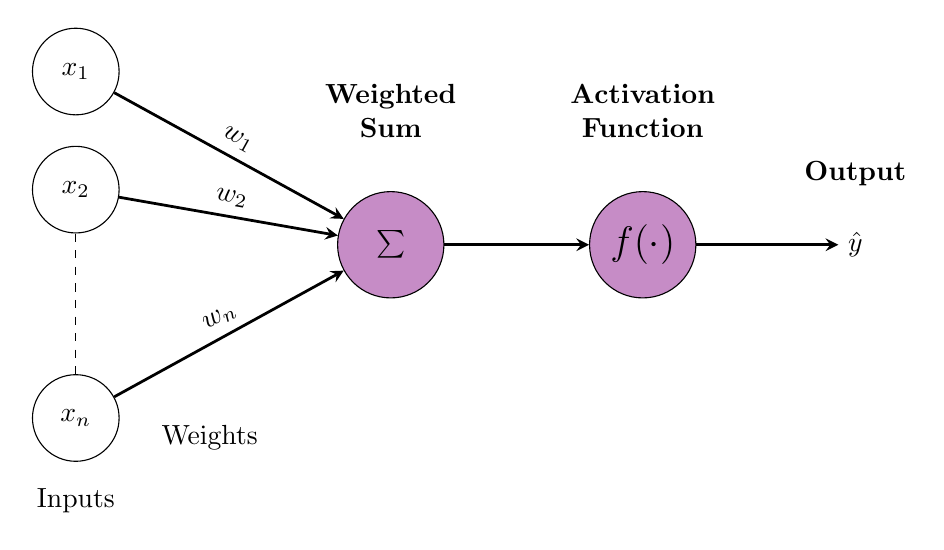
\begin{tikzpicture}[
    node distance=1.8cm,
    neuron/.style={circle, draw, minimum size=1.1cm, font=\bfseries},
    block/.style={circle, draw, fill=violet!45, minimum size=1.35cm},
    arrow/.style={->, >=stealth, line width=1pt},
    label/.style={font=\bfseries}
]

% Inputs
\node[neuron] (x1) at (0,2.2) {$x_1$};
\node[neuron] (x2) at (0,0.7) {$x_2$};
\node[neuron] (xn) at (0,-2.2) {$x_n$};

\draw[dashed] (x2) -- (xn);

\node at (0,-3.25) {Inputs};

% Weighted sum
\node[block] (sum) at (4,0) {\Large $\sum$};
\node[label, align=center] at (4,1.7) {Weighted\\Sum};

% Activation function
\node[block] (act) at (7.2,0) {\Large $f(\cdot)$};
\node[label, align=center] at (7.2,1.7) {Activation\\Function};

% Output
\node[label] (outlabel) at (9.9,0.9) {Output};
\node (out) at (9.9,0) {$\hat{y}$};

% Arrows from inputs
\draw[arrow] (x1) -- node[above, sloped] {$w_1$} (sum);
\draw[arrow] (x2) -- node[above, sloped] {$w_2$} (sum);
\draw[arrow] (xn) -- node[above, sloped] {$w_n$} (sum);

% Arrows between processing nodes
\draw[arrow] (sum) -- (act);
\draw[arrow] (act) -- (out);

% Weights label
\node at (1.7,-2.45) {Weights};

\end{tikzpicture}%
    }
    \caption{Single artificial neuron: weighted sum of inputs $x_i$, bias absorbed
    into weights if a constant input is used, nonlinear activation $\sigma$,
    and scalar output $\hat{y}$ (cf.\ Equation above with $\sigma = f$).}
    \label{fig:perceptron}
\end{figure}

A \emph{multilayer perceptron} (MLP) stacks $L$ layers of neurons.  Writing
$\mathbf{h}^{(0)} = \mathbf{x}$ for the input, each hidden layer computes
%
\begin{equation}
    \mathbf{h}^{(l)} = \sigma\!\left(W^{(l)}\mathbf{h}^{(l-1)} + \mathbf{b}^{(l)}\right),
    \quad l = 1, \ldots, L,
\end{equation}
%
where $W^{(l)}$ and $\mathbf{b}^{(l)}$ are the weight matrix and bias vector
of layer $l$.  The final layer produces the network output, which may be a
vector of logits (for a discrete distribution), the parameters of a
continuous distribution (e.g.\ mean and log-standard-deviation for a Gaussian
policy), or a scalar (for a value estimate).  The universal approximation
theorem guarantees that a single sufficiently wide hidden layer can approximate
any continuous function on a compact domain to arbitrary precision~\cite{goodfellow2016deep},
although in practice depth is more parameter-efficient than width.
Figure~\ref{fig:mlp} shows a representative fully-connected depth (three
hidden layers).

\begin{figure}[ht]
    \centering
    \resizebox{0.88\linewidth}{!}{%
        % In the preamble:
% \usepackage{tikz}
% \usetikzlibrary{arrows.meta}

\begin{tikzpicture}[
    neuron/.style={
        circle,
        draw=black,
        line width=0.9pt,
        minimum size=9mm
    },
    input neuron/.style={
        neuron,
        fill=blue!15
    },
    hidden neuron/.style={
        neuron,
        fill=green!15
    },
    output neuron/.style={
        neuron,
        fill=red!15
    },
    conn/.style={
        -{Latex[length=2mm]},
        draw=gray!100,
        line width=0.7pt
    },
    io/.style={
        -{Latex[length=2mm]},
        draw=black,
        line width=0.9pt
    },
    label/.style={
        font=\footnotesize,
        text=black
    }
]

% ------------------------------------------------
% Input arrows
% ------------------------------------------------
\draw[io] (-0.9,  1.4) -- (0.45,  1.4);
\draw[io] (-0.9,  0.0) -- (0.45,  0.0);
\draw[io] (-0.9, -1.4) -- (0.45, -1.4);

\node[label] at (-1.6,0) {Inputs};

% ------------------------------------------------
% Input layer
% ------------------------------------------------
\node[input neuron]  (I1) at (1.0,  1.4) {};
\node[input neuron]  (I2) at (1.0,  0.0) {};
\node[input neuron]  (I3) at (1.0, -1.4) {};

% ------------------------------------------------
% Hidden layer 1
% ------------------------------------------------
\node[hidden neuron] (H11) at (2.9,  2.1) {};
\node[hidden neuron] (H12) at (2.9,  0.7) {};
\node[hidden neuron] (H13) at (2.9, -0.7) {};
\node[hidden neuron] (H14) at (2.9, -2.1) {};

% ------------------------------------------------
% Hidden layer 2
% ------------------------------------------------
\node[hidden neuron] (H21) at (4.8,  2.1) {};
\node[hidden neuron] (H22) at (4.8,  0.7) {};
\node[hidden neuron] (H23) at (4.8, -0.7) {};
\node[hidden neuron] (H24) at (4.8, -2.1) {};

% ------------------------------------------------
% Hidden layer 3
% ------------------------------------------------
\node[hidden neuron] (H31) at (6.7,  2.1) {};
\node[hidden neuron] (H32) at (6.7,  0.7) {};
\node[hidden neuron] (H33) at (6.7, -0.7) {};
\node[hidden neuron] (H34) at (6.7, -2.1) {};

% ------------------------------------------------
% Output layer
% ------------------------------------------------
\node[output neuron] (O1) at (8.6,  0.7) {};
\node[output neuron] (O2) at (8.6, -0.7) {};

% ------------------------------------------------
% Connections: input -> hidden 1
% ------------------------------------------------
\foreach \i in {I1,I2,I3}
    \foreach \j in {H11,H12,H13,H14}
        \draw[conn] (\i) -- (\j);

% Hidden 1 -> hidden 2
\foreach \i in {H11,H12,H13,H14}
    \foreach \j in {H21,H22,H23,H24}
        \draw[conn] (\i) -- (\j);

% Hidden 2 -> hidden 3
\foreach \i in {H21,H22,H23,H24}
    \foreach \j in {H31,H32,H33,H34}
        \draw[conn] (\i) -- (\j);

% Hidden 3 -> output
\foreach \i in {H31,H32,H33,H34}
    \foreach \j in {O1,O2}
        \draw[conn] (\i) -- (\j);

% ------------------------------------------------
% Output arrows
% ------------------------------------------------
\draw[io] (O1) -- (10.0,  0.7);
\draw[io] (O2) -- (10.0, -0.7);

\node[label] at (10.7,0) {Outputs};

% ------------------------------------------------
% Layer labels
% ------------------------------------------------
\node[label] at (1.0,-2.95) {Input Layer};
\node[label] at (4.8,-3.25) {Hidden Layers};
\node[label] at (8.6,-2.95) {Output Layer};

\end{tikzpicture}
%
    }
    \caption{Fully-connected feed-forward network: input layer, three hidden
    layers, and output layer.  The actor and critic in this work use separate
    \glspl{mlp} of this form.}
    \label{fig:mlp}
\end{figure}

Network parameters are collected into a vector $\theta$ and optimized by
minimizing a loss function $\mathcal{L}(\theta)$ via stochastic gradient
descent or one of its adaptive variants (Adam, RMSProp).  The gradient
$\nabla_\theta \mathcal{L}$ is computed efficiently by
\emph{backpropagation}, which applies the chain rule layer by layer from the
output back to the inputs~\cite{goodfellow2016deep}.  In the RL setting
discussed in Section~\ref{sec:rl}, the loss is derived from the policy
objective $J(\theta)$ and the critic's value-prediction error, so the same
backpropagation machinery drives both the actor and critic updates.

\subsection{Deep Learning}

\emph{Deep learning} refers to the use of neural networks with many hidden
layers.  Greater depth allows the network to compose simple transformations
into increasingly abstract representations: early layers typically capture
low-level features while later layers encode task-relevant structure.  This
hierarchical inductive bias has proven effective across perception, language,
and control, including in high-dimensional continuous-control settings
directly comparable to this work~\cite{silver2016mastering,berner2019dota}.

For the \gls{vsss} policy, the observation vector includes the positions,
orientations, and velocities of all robots and the ball — the full simulator
state — so no hidden dynamics need to be inferred from a history of frames.
Recurrent architectures are therefore unnecessary; a feed-forward network
suffices.  A fully-connected
\gls{mlp} with two or three hidden layers captures the required nonlinear
dependencies while remaining fast to evaluate on a \gls{gpu} across thousands
of parallel environments.  The actor and critic each use a separate
\gls{mlp}; sharing lower layers is possible but not assumed in the baseline
design.

Two practical techniques are relevant to stability in deep \gls{rl}.  First,
layer normalization~\cite{goodfellow2016deep} standardizes activations within
each layer, reducing sensitivity to the scale of inputs and mitigating the
non-stationarity of the input distribution that arises because the policy
changes throughout training.  Second, the outputs of the final actor layer
are initialized with small weights so that the policy starts close to a
uniform distribution, allowing the agent to explore broadly early in
training.  Both choices are standard in the \gls{ppo} implementations applied
to continuous-control domains.

\section{Reinforcement Learning}
\label{sec:rl}

\subsection{Fundamentals}

Reinforcement learning formalizes sequential decision-making as interaction
between an agent and an environment~\cite{sutton2018reinforcement}.  In the
Markov decision process (\gls{mdp}) formulation, the environment is described
by the tuple $\langle \mathcal{S}, \mathcal{A}, \mathcal{P}, R, \gamma
\rangle$, where $\mathcal{S}$ is the state space, $\mathcal{A}$ is the action
space, $\mathcal{P}(s_{t+1} \mid s_t, a_t)$ is the transition distribution,
$R$ is the reward function, and $\gamma \in [0,1]$ is the discount factor.

The agent acts according to a policy $\pi_\theta$ parameterized by $\theta$.
Its objective is to maximize the expected discounted return:
%
\begin{equation}
    J(\theta) = \mathbb{E}_{\pi_\theta}\!\left[\sum_{t=0}^{T} \gamma^t
    r_t\right].
\end{equation}
%
Value functions summarize long-term quality.  The state-value function
$V^\pi(s)$ gives the expected return from state $s$ under $\pi$, and the
action-value function $Q^\pi(s,a)$ conditions additionally on taking action
$a$.  The advantage function,
%
\begin{equation}
    A^\pi(s,a) = Q^\pi(s,a) - V^\pi(s),
\end{equation}
%
measures how much better or worse a particular action is relative to the
policy's average behavior in that state.  This quantity appears centrally in
the policy-gradient and actor-critic methods described below.

\subsection{Policy Gradient, Actor-Critic, and PPO}

Policy-gradient methods optimize $\pi_\theta$ directly via gradient ascent on
$J(\theta)$.  The standard estimator is
%
\begin{equation}
    \nabla_\theta J(\theta) =
    \mathbb{E}\!\left[
        \nabla_\theta \log \pi_\theta(a_t \mid s_t)\,\hat{A}_t
    \right],
    \label{eq:pg}
\end{equation}
%
where $\hat{A}_t$ is a sampled estimate of the advantage.  The estimator is
unbiased but can exhibit high variance, which makes learning slow or unstable.
Actor-critic methods reduce this variance by learning a parametric critic
$V_w(s)$ alongside the policy.  The critic supplies the baseline needed to
compute $\hat{A}_t$ via Generalized Advantage Estimation
(GAE)~\cite{schulman2015gae}:
%
\begin{equation}
    \hat{A}_t^{\mathrm{GAE}} = \sum_{k=0}^{T-t}(\gamma\lambda)^k\,\delta_{t+k},
    \qquad
    \delta_t = r_t + \gamma V_w(s_{t+1}) - V_w(s_t),
    \label{eq:gae}
\end{equation}
%
where $\lambda \in [0,1]$ trades variance against bias: $\lambda \to 0$
relies heavily on the critic estimate, and $\lambda \to 1$ relies more on
actual returns.

\gls{ppo}~\cite{schulman2017ppo} extends the actor-critic framework with a
constraint that prevents destructively large policy updates.  It defines the
probability ratio $r_t(\theta) = \pi_\theta(a_t \mid s_t) /
\pi_{\theta_\mathrm{old}}(a_t \mid s_t)$ and optimizes the clipped surrogate
objective:
%
\begin{equation}
    L^{\mathrm{CLIP}}(\theta) =
    \mathbb{E}\!\left[
        \min\!\left(
            r_t(\theta)\,\hat{A}_t,\;
            \mathrm{clip}\!\left(r_t(\theta),\,1-\varepsilon,\,1+\varepsilon\right)
            \hat{A}_t
        \right)
    \right].
    \label{eq:ppo}
\end{equation}
%
The clipping parameter $\varepsilon$ bounds how far $\pi_\theta$ may deviate
from the behavior policy that collected the data, removing the incentive to
take excessively large gradient steps.  Because a single batch can be reused
for several gradient epochs before being discarded, \gls{ppo} achieves better
sample efficiency than a plain policy-gradient update while remaining simpler
to implement than \gls{trpo}~\cite{schulman2015trpo}.


Its robustness across the \gls{vsss} domain~\cite{tg_thiago,tg_thay,brandao2022} make it the
natural algorithm choice for this work.

% ------------------------------------------------------------------
\subsection{Curriculum Learning}
% ------------------------------------------------------------------

Curriculum learning organizes the training process as a sequence of tasks of
increasing difficulty, rather than exposing the agent to the final task from
the start~\cite{bengio2009curriculum}.  The motivation is practical: in
settings with sparse rewards or a large initial performance gap between random
and competent behavior, a policy initialized at random may never encounter
enough informative signal to make progress.  A curriculum provides a ramp that
keeps the task at a difficulty where learning can occur.

For \gls{vsss}, the final objective — winning 3v3 matches — is far too complex
for a randomly-initialized policy to explore productively.  A staged approach
addresses this: allied robots first practice ball conduction and basic
positioning without any opposition, then face opponents only once those
sub-skills are established.

% ------------------------------------------------------------------
\subsection{Prioritized Level Replay}
% ------------------------------------------------------------------

\gls{plr}~\cite{prioritized_level_replay} is a mechanism for allocating training
experience across a distribution of situations, or \emph{levels}, according to
an estimate of their future learning potential rather than uniformly at random.
The core observation is that, at any point in training, some situations will
be either too easy (the agent already solves them reliably) or too hard
(the agent cannot yet extract any useful gradient).  The most informative
situations are those at the boundary of current competence.

After each episode on level $l_i$, \gls{plr} computes a score
%
\begin{equation}
    S_i = \frac{1}{T}\sum_{t=0}^{T}\bigl|\hat{A}_t^{\mathrm{GAE}}\bigr|,
    \label{eq:plr_score}
\end{equation}
%
the mean absolute \gls{gae} over the trajectory~\cite{prioritized_level_replay}.  This
quantity is equivalent to the mean $L_1$ value loss under \gls{ppo}, and
levels on which the critic is most surprised carry the highest priority.  A
staleness correction down-weights levels that have not been visited recently,
preventing the replay distribution from becoming stale with respect to a
policy that has since improved.  The resulting sampling distribution
$P_{\mathrm{replay}}$ interpolates between high-priority (high value-error)
and unseen levels, inducing an implicit curriculum without requiring prior
knowledge of level difficulty.

In the context of this thesis, a level is a game initialization: robot poses,
ball position, velocities, and any relevant game-state context.  Because
\gls{vsss} admits a large space of initial configurations with very unequal
learning value, \gls{plr} is a natural fit.  The high-throughput simulator
developed here makes the approach practical: with enough parallel environments,
the overhead of maintaining a priority buffer and replaying specific
initializations is negligible compared to the benefit of directing more
experience toward informative situations.

% ------------------------------------------------------------------
\subsection{Multi-Agent Reinforcement Learning and Self-Play}
% ------------------------------------------------------------------

When several policies act in the same environment, the standard single-agent
\gls{mdp} formulation no longer fully characterizes the learning problem.  Each
agent's optimal policy depends on the behavior of the others, which themselves
change during training — a property known as non-stationarity.  In cooperative
settings this manifests as a credit-assignment problem: individual contributions
to a shared reward are difficult to attribute.  In competitive settings, the
moving target created by an improving opponent can destabilize learning.  Robot
soccer combines both regimes within the same episode.

Self-play addresses the competitive aspect by using the agent itself — or
previously saved versions — as the opponent.  The opponent automatically
becomes harder as the agent improves, creating a natural difficulty curriculum.
However, training exclusively against the latest version of the policy can lead
to \emph{strategy collapse}: the agent discovers a local best-response that
dominates the current opponent but is easily exploited by a broader range of
strategies.  Fictitious self-play~\cite{brown1951fsp} mitigates this by playing
against a mixture over all historical policies, with convergence guarantees for
two-player zero-sum games.  In practice, emphasizing more recent opponents
while retaining some probability on older ones achieves a good balance between
generalization and training efficiency — the family of opponent-sampling
schemes studied by \cite{master_thay} and the league-training approach of
\cite{starcraft_marl} are both instances of this principle.

\gls{ctde} is a standard architecture for cooperative teams: during training,
each agent's critic may access global state to produce more accurate value
estimates, while the policies themselves are conditioned only on locally
available observations.  At execution time the critics are discarded, and each
robot acts from its own observation alone.  This separation allows the critic
to leverage information that would not be available in deployment without
constraining the policy to require it.

% ------------------------------------------------------------------
\subsection{Exploiting Symmetry in the VSSS Problem}
% ------------------------------------------------------------------

The 3v3 \gls{vsss} setting has two classes of symmetry that can be exploited
to improve learning efficiency.

\textbf{Permutation symmetry.}  The three robots on the same team are
homogeneous: they have identical kinematics and contribute to the same team
objective.  The value of a team state should therefore be invariant to which
robot is labeled 1, 2, or 3.  Sharing policy and critic parameters across all
three robots exploits this directly — a single network is updated using
transitions from all three agents simultaneously, tripling effective data
throughput without requiring a larger batch.  \textcite{brandao2022} applied
exactly this principle in their \gls{vsss} multi-agent formulation, observing
that shared parameters provide a natural implicit regularization.

\textbf{Reflection symmetry.}  The VSSS field is bilaterally symmetric about
its longitudinal axis.  A game state mirrored across that axis, with signs of
transverse coordinates flipped consistently for positions, velocities, and
actions, is an equally valid game state with the same value.  This symmetry
can be exploited through data augmentation: every collected transition generates
a second, reflected transition at no additional simulation cost, doubling the
effective number of distinct states the policy is trained on.

Both forms of symmetry are treated as first-class design choices in the
training methodology rather than as optional post-processing.

% ------------------------------------------------------------------
\section{High-Throughput, GPU-Accelerated Simulation}
% ------------------------------------------------------------------

On-policy algorithms like \gls{ppo} repeatedly collect fresh rollouts and
discard them after a single round of updates.  The number of environment steps
per wall-clock second is therefore a direct multiplier on how much training
progress can be made in a given time budget.  When the simulator is the
bottleneck, improvements to the learning algorithm yield diminishing returns.

\gls{jax}~\cite{jax2018github} provides three complementary transformations
that make GPU-parallel simulation practical.  \texttt{jit} compiles a
numerical function to native code, eliminating Python overhead.  \texttt{vmap}
lifts a single-environment step into a vectorized step over a batch of
environments, enabling thousands of independent games to advance in a single
device call.  \texttt{scan} implements a fixed-length loop (a rollout horizon)
as a single compiled operation, avoiding repeated Python-level dispatch.
Because \gls{jax} programs are purely functional, state is passed explicitly
with no hidden side-effects, so the entire collect-and-update loop runs on the
accelerator without data copies between host and device.

For \gls{vsss}, the physics model — rigid-body kinematics, elastic wall
collisions, and a friction model for ball--floor contact — is simple enough
to implement as differentiable array operations without any approximation that
would matter for policy learning.